% This template was initially provided by Dulip Withanage.
% Modifications for the database systems research group
% were made by Conny Junghans,  Jannik Strötgen and Michael Gertz

\documentclass[
     12pt,         % font size
     a4paper,      % paper format
     BCOR10mm,     % binding correction
     DIV14,        % stripe size for margin calculation
     ]{article}

%%%%%%%%%%%%%%%%%%%%%%%%%%%%%%%%%%%%%%%%%%%%%%%%%%%%%%%%%%%%

% PACKAGES:

% Use German :
\usepackage[english]{babel}
% Input and font encoding
\usepackage[latin1]{inputenc}
\usepackage[T1]{fontenc}
% Index-generation
\usepackage{makeidx}
% Einbinden von URLs:
\usepackage{url}
% Special \LaTex symbols (e.g. \BibTeX):
%\usepackage{doc}
% Include Graphic-files:
\usepackage{graphicx}
% Include doc++ generated tex-files:
%\usepackage{docxx}

% Fuer anderthalbzeiligen Textsatz
\usepackage{setspace}

% hyperrefs in the documents
\PassOptionsToPackage{hyphens}{url}\usepackage[bookmarks=true,colorlinks,pdfpagelabels,pdfstartview = FitH,bookmarksopen = true,bookmarksnumbered = true,linkcolor = black,plainpages = false,hypertexnames = false,citecolor = black,urlcolor=black]{hyperref}
%\usepackage{hyperref}

%%%%%%%%%%%%%%%%%%%%%%%%%%%%%%%%%%%%%%%%%%%%%%%%%%%%%%%%%%%%

% OTHER SETTINGS:

% Choose language
\newcommand{\setlang}[1]{\selectlanguage{#1}\nonfrenchspacing}


\begin{document}

% TITLE:
\pagenumbering{roman} 
\begin{titlepage}


\vspace*{1cm}
\begin{center}
\vspace*{3cm}
\textbf{ 
\Large Heidelberg University\\
\smallskip
\Large Institute of Computer Science\\
\smallskip
\Large Database Systems Research Group\\
\smallskip
}

\vspace{3cm}

\textbf{\large Project Proposal for the lecture Text Analytics}

\vspace{0.5\baselineskip}
{\huge
\textbf{Working Title}
}
\end{center}

\vfill 

{\large
\begin{tabular}[l]{ll}
Team Member: & Name, Matriculation Number, Course of Study\\
  & email address\\
Team Member: & Name, Matriculation Number, Course of Study\\
  & email address\\
Team Member: & Name, Matriculation Number, Course of Study\\
  & email address\\

% If the line goes too far to the right, you can alter this slightly, e.g.
Team Member: & Very long Name, Matriculation Number\\
  & Course of Study, email address\\
  
\end{tabular}
}

\end{titlepage}

\pagenumbering{arabic} 

\section{Introduction}
Motivate your project and state the \textit{real-world problem} you want to solve.

\section{Section}

Use sections to organize your contents. Read the project proposal guidelines available on Moodle to get more information on the contents your proposal should cover. Do not forget to cite online sources~\cite{WFR2017}, books~\cite{goldberg2017neural} or articles you are referencing! It may also be useful to integrate charts or figures in your proposal as seen in Figure~\ref{fig:example}.

\begin{figure}[h]
  \centering
  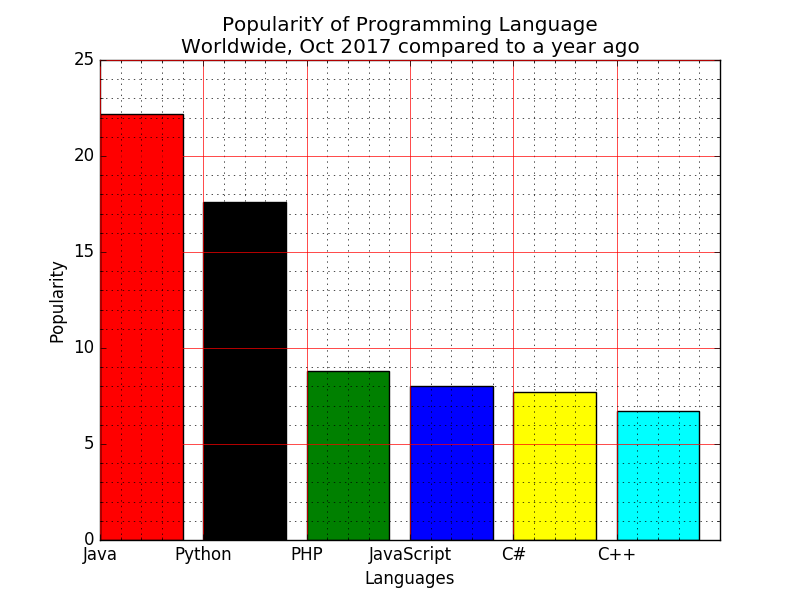
\includegraphics[scale=0.3]{figures/example_barchart}
  \caption[]{An example chart showing the change of popularity of various programming languages\footnotemark[1].}
  \label{fig:example}
\end{figure}

\footnotetext[1]{\url{https://www.w3resource.com/w3r_images/matplotlib-barchart-exercise-4.png}}

In the Latex source provided together with this PDF, you also find hints on how to work on one Latex project collaboratively.


%%%%%%%%%%%%%%%%%%%%%%%%%%%%%%%%%%%%%%%%%%%%%%%%%%%%%%%%%%%%

% The following is especially useful if you work together on one proposal or report, and want to alter its content independently from each other (e.g., to keep your commit history clean).

% Alternative: put content in separate files
% Check the difference between including these files using \input{filename} and \include{filename} and see which one you like better
%\chapter{Einleitung}\label{intro}
%\section{Introduction}

One current research area in the field of text analytics is hate speech detection. Many approaches from the recent past take use of neural network architectures to deal with such classification problems. One of the most common approaches is to use uni- and bidirectional long short-term memory (LSTM) networks, a recurrent neural network architecture that can process input of arbitrary length and remembers context information \cite{Dorris2020, Syam2019, Saksesi2018}. The paper \cite{Founta2019} states, that even a simple gated recurrent unit (GRU) architecture can perform as good as more complex units. \cite{Saleh2020} repurposes the famous bidirectional encoder representations from transformers (BERT) language model to perform classification tasks for hate speech detection. Besides that, other approaches use convolutional neural networks (CNNs) to extract typical hate speech patterns \cite{Badjatiya2017, Roy2020, Kapil2020} or even deep belief network algorithms \cite{Muhammad2020}. Using neural network approaches means to automatically learn representative features for the classification task. On the other hand, the papers introduced in \autoref{related_work} use a different approach by solving the classification task with manually extracted features. Nevertheless, none of the papers combines the different achievements of such recent research and compares it to a baseline neural network architecture, which is what this work is dedicated to.

After a definition of the term \enquote{hate speech} in \autoref{approach} different classifiers will be trained on a holistic, hand-crafted feature set based on recent publications in the field of hate speech detection. The task includes building and preprocessing a training corpus as well as introducing and explaining the different kinds of features. How well the different classifiers perform compared to a neural network approach as a baseline and several statictical insights into typical hate speech artifacts will be presented in \autoref{results}. The results of this work in \autoref{analysis} should show which features work best for which classifier and which problems can be addressed with conventional machine learning methods and which not as opposed to neural network approaches. A summary over the achievements earned will be drawn in \autoref{conclusion}.
%
%\chapter{Voraussetzungen}\label{bg}
%\input{background}

%%%%%%%%%%%%%%%%%%%%%%%%%%%%%%%%%%%%%%%%%%%%%%%%%%%%%%%%%%%%

% References (Literaturverzeichnis):
% see
% https://de.wikibooks.org/wiki/LaTeX-W%C3%B6rterbuch:_bibliographystyle
% for the different formats and styles

\bibliographystyle{plain}
% b) The File:
\bibliography{references}

\end{document}
